\subsection{Deep Learning}

El Deep Learning o Aprendizaje Profundo es una rama del Machine Learning que conforma varios tipos de algoritmos y enfoques mucho más amplios. Este involucra tratar a los problemas que requiere mayor generalización como lo es la visión por computadora y el reconocimiento de voz. Es decir, estos problemas generales se refieren a problemas que los humanos pueden resolver con facilidad. El Deep Learning involucra al Aprendizaje Supervisado, No Supervisado y el Aprendizaje por Refuerzo. El concepto de “profundidad” se refiere a la característica de sus enfoques en usar muchas capas de redes neuronales artificiales, donde cada una de estas realiza una operación especial, para que en conjunto su complejidad y potencia de resolución de problemas sea mayor. \parencite{bk_hurbans2020grokking}

En el caso de esta investigación, una de las técnicas del Deep Learning a usar son las Convoluciones. Esta técnica permite la extracción de características de imágenes para posteriormente realizar su clasificación con respecto a estos. En el proceso de convolución es importante mencionar a los filtros. Estos contienen pesos que son multiplicados por los valores de los pixeles de una imagen, para que finalmente se obtenga un nuevo valor de pixel \parencite{bk_moroney2020aiandml}. A continuación, se presenta un ejemplo gráfico de convolución 2D en una imagen del conjunto de datos Fashion MNIST.

\begin{figure}[H]
	\begin{center}
		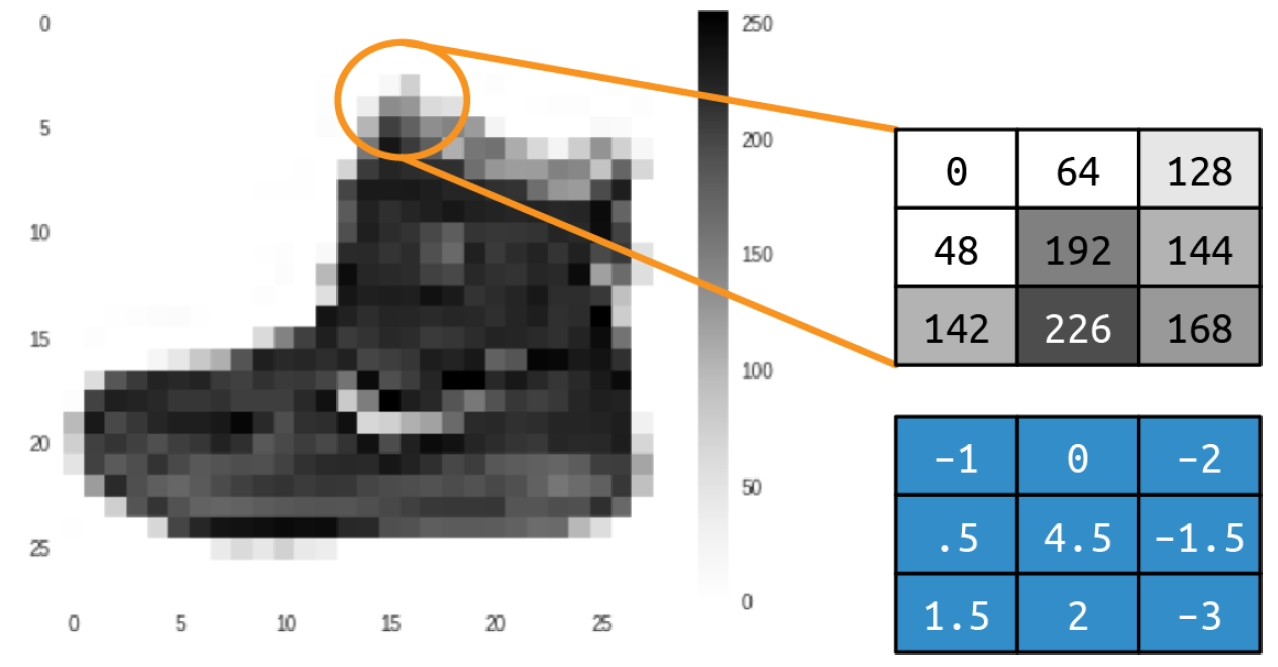
\includegraphics[width=0.80\textwidth]{2/figures/cnn_fash_mnist.png}
		\caption[Convolución de imagen de Fashion MNIST]{Convolución de imagen de Fashion MNIST. \\
		Fuente: \cite{bk_moroney2020aiandml}. \textit{AI and Machine Learning for Coders}.}
		\label{2:fig201}
	\end{center}
\end{figure}

Con un filtro de 3x3 como se muestra en la imagen, se puede modificar el valor del pixel. Este proceso se repite con cada pixel en imagen. Finalmente, se obtiene una imagen nueva conocida como una imagen filtrada. \parencite{bk_moroney2020aiandml} En el ejemplo anterior, el nuevo valor del pixel original 192 será 577, pues este es el resultado de multiplicar, y posteriormente sumar, los pesos del filtro con el valor del pixel y sus vecinos.

Existen distintos tipos de filtros que modifican y otorgan distintos tipos de resultados. Como ejemplo se presentan a continuación las siguientes imágenes.

\begin{figure}[H]
	\begin{center}
		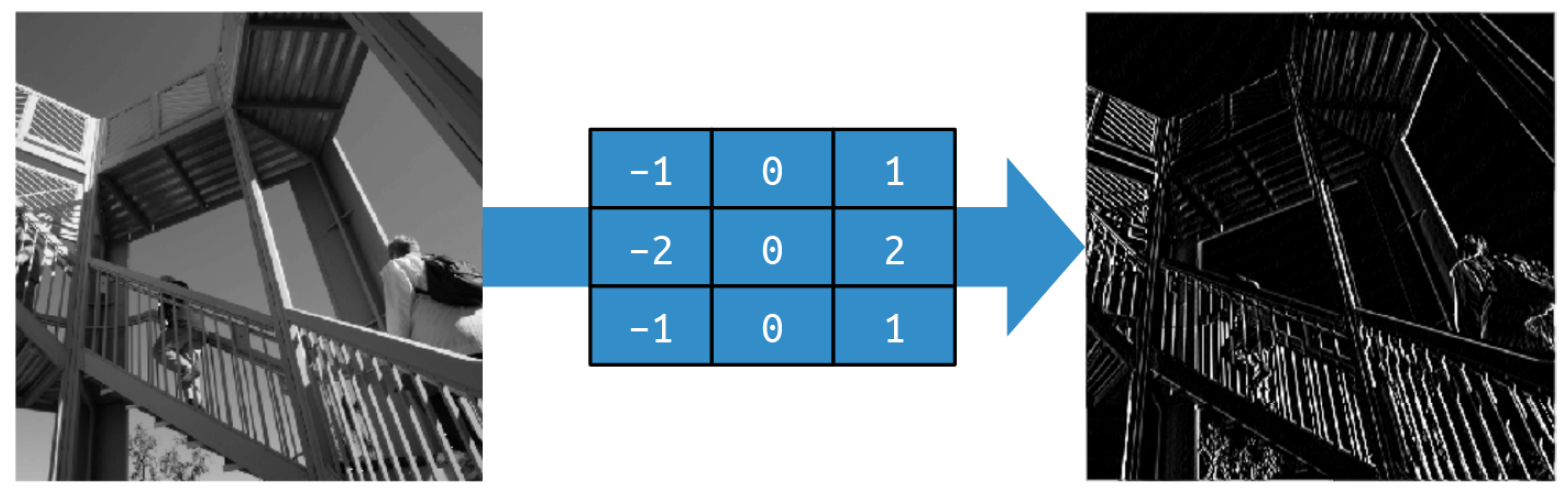
\includegraphics[width=1.00\textwidth]{2/figures/cnn_filtro_vert.png}
		\caption[Convolución de imagen con filtro de líneas verticales]{Convolución de imagen con filtro de líneas verticales. \\
		Fuente: \cite{bk_moroney2020aiandml}. \textit{AI and Machine Learning for Coders}.}
		\label{2:fig202}
	\end{center}
\end{figure}

\begin{figure}[H]
	\begin{center}
		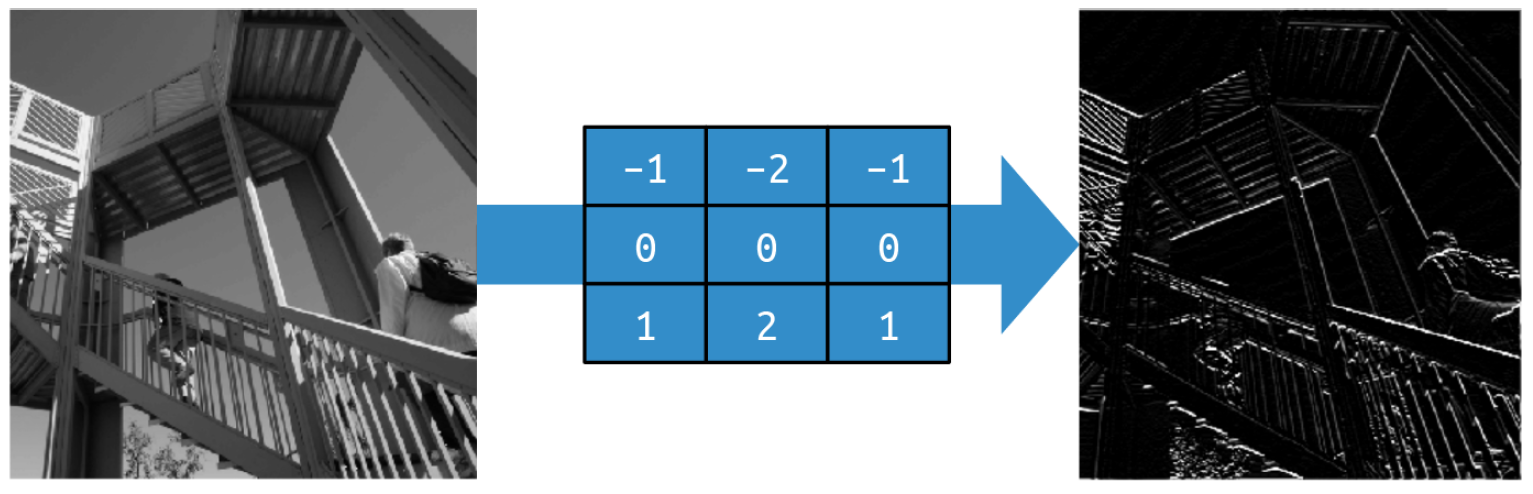
\includegraphics[width=1.00\textwidth]{2/figures/cnn_filtro_hori.png}
		\caption[Convolución de imagen con filtro de líneas horizontales]{Convolución de imagen con filtro de líneas horizontales. \\
		Fuente: \cite{bk_moroney2020aiandml}. \textit{AI and Machine Learning for Coders}.}
		\label{2:fig203}
	\end{center}
\end{figure}

El primer filtro realiza modificaciones a una imagen original para finalmente obtener otra imagen distinta en donde se resaltan las líneas verticales. Caso contrario pasa con el segundo filtro, donde la imagen original es modificada para resaltar sus líneas horizontales. Así, existen distintos tipos de filtros con distintos pesos. Cada uno de estos permite resaltar en las imágenes, a través de modificaciones en sus pixeles, sus características más importantes que serán de utilidad para diferenciar entre una clase u otra de un conjunto de imágenes. También se podría decir que esta técnica de aplicar convoluciones permite reducir la cantidad de información presente en las imágenes, entonces se podría aprender o encontrar un conjunto de filtros específicos capaces de reducir la gran cantidad de información de las imágenes en características que estén relacionadas a sus respectivas etiquetas \parencite{bk_moroney2020aiandml}.

Para reducir la cantidad de información presente en las imágenes, manteniendo al mismo tiempo las características obtenidas por las convoluciones, es necesario aplicar otra técnica entro del mundo del Deep Learning.

El proceso de pooling consiste en eliminar cierta cantidad de pixeles en una imagen, mientras se mantienen las partes resaltantes de la misma. Este proceso normalmente se realiza con agrupaciones de 2x2 en los pixeles de una imagen. Estas agrupaciones también son conocidos como pool. Dentro de cada uno de estas se selecciona el máximo valor de pixel. El proceso se repite con nuevos grupos de pixeles para finalmente obtener una nueva imagen de tamaño considerablemente reducido. \parencite{bk_moroney2020aiandml} A continuación se presenta un ejemplo gráfico.

\begin{figure}[H]
	\begin{center}
		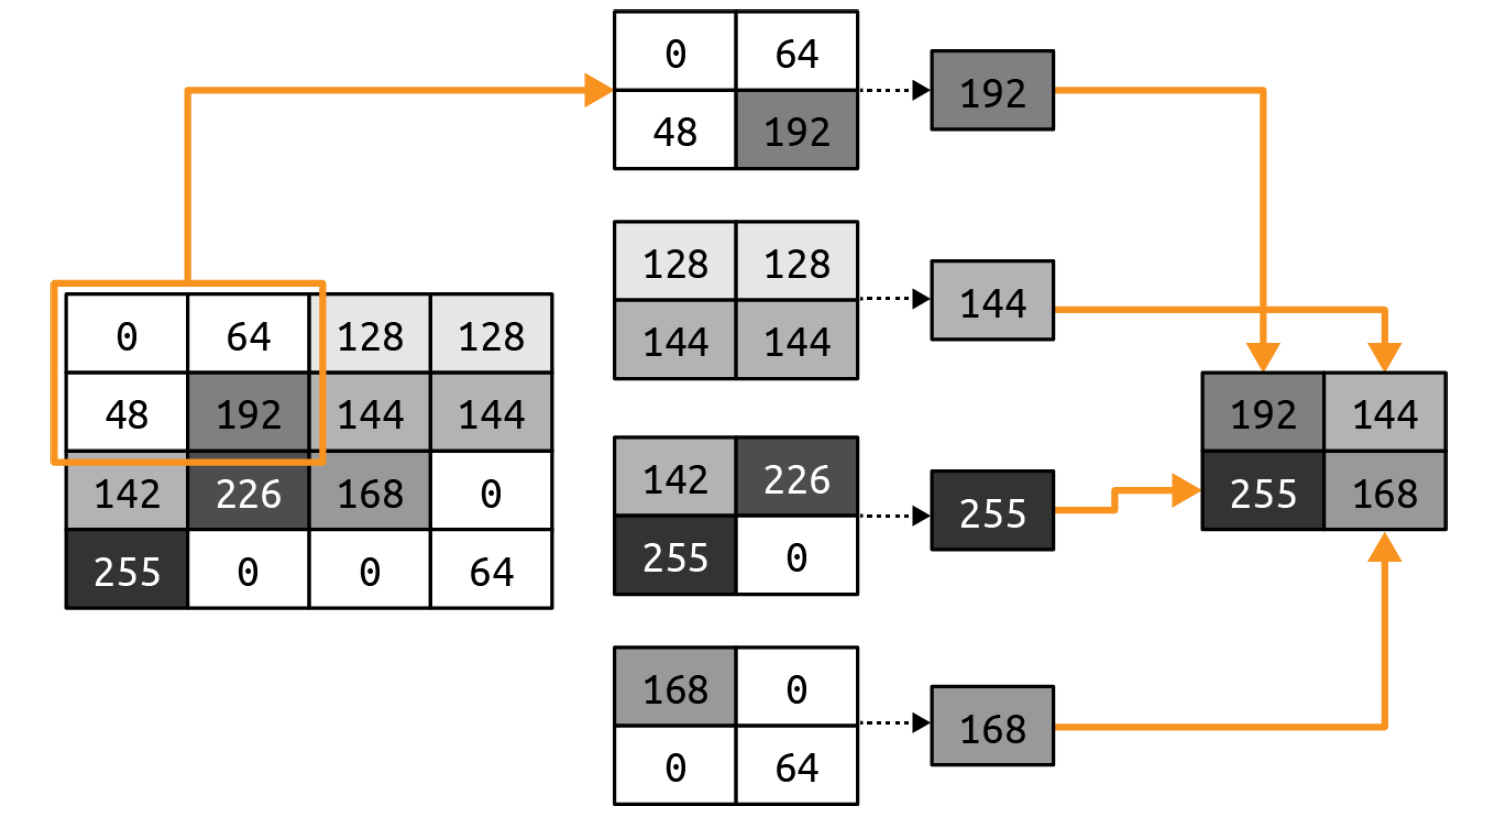
\includegraphics[width=0.85\textwidth]{2/figures/cnn_pool_examp.png}
		\caption[Ejemplo de max-pooling con un pool de 2x2]{Ejemplo de max-pooling con un pool de 2x2. \\
		Fuente: \cite{bk_moroney2020aiandml}. \textit{AI and Machine Learning for Coders}.}
		\label{2:fig204}
	\end{center}
\end{figure}

La imagen original de 4x4 pixeles, luego de ser aplicado el proceso de pooling, se obtiene una imagen reducida de 2x2 pixeles. De manera general, la imagen redujo a la cuarta parte de la cantidad original de pixeles.

Con estas dos técnicas del Deep Learning se han ido desarrollando distintas arquitecturas de redes neurales en la última década. Algunas más complejas y con más capas que otras. Cada una de estas han logrado desempeñarse de forma satisfactoria con el conjunto de datos con el que se han entrenado, demostrando el gran potencial de la redes neuronales convolucionales o CNN.

Algunas de las arquitecturas más conocidas y que han sido usadas en gran variedad de investigaciones son los VGG, ResNet, Inception y DenseNet.

La arquitectura VGG o VGGNet es una red neuronal artificial con una profundidad de 16 o 19 capas (dependiendo de la versión que se analice) y usa pequeños filtros de convolución de tamaño 3x3 a través de estas. Este modelo participó en el ImageNet Challenge 2014, donde logró el primer puesto en las tareas de localización y segundo puesto en clasificación. Además, tiene la alta capacidad de generalización en otros conjuntos de datos, es decir, es capaz de obtener buenos resultados con imágenes distintas a las usadas para su entrenamiento. \parencite{pr_simonyan2015vdcn}

Otra arquitectura bastante difundida en el mundo del Deep Learning y las CNN es ResNet. Esta arquitectura nace de la premisa del aumento de la dificultad de entrenar las redes neuronales profundas. Con el objetivo de facilitar este proceso se añade a las ya conocidas CNN el concepto de residual, para obtener redes residuales que sean mucho más fáciles de optimizar y capaces de obtener mejor desempeño a más grande sea la profundidad de la red. El modelo tuvo 152 capas, ocho veces más grande que las arquitecturas VGG, y fue evaluada con el conjunto de datos ImageNet. \parencite{pr_he2016deepres}

Inception es una arquitectura que obtuvo un alto desempeño en las tareas de clasificación y detección en el ImageNet Large-Scale Visual Recognition Challenge 2014 (ILSVRC14). La principal distinción de este modelo es el uso de los recursos informáticos a través de la red. Esto significa que mientras más aumente la complejidad del modelo a través de su profundidad, los recursos computacionales no variarán a gran escala como se esperaría. Esto se logra a través del uso de módulos de Inception en algunas capas de la arquitectura en general. Los distintos módulos se encuentran apilados unos sobre otros y con algunas capas max-pooling. Dentro de esta arquitectura, se tiene a GoogLeNet, que no es más que una versión de Inception de 22 capas (este modelo fue el presentado a ILSVRC14). \parencite{pr_szegedy2015goingdwc}

DenseNet nace con la premisa de que las CNN pueden obtener mejores desempeños si se tienen conexiones cortas entre las capas cerca de la entrada y salida de la red. La propuesta de esta red consiste en establecer una conexión de cada capa con todas las demás capas de la misma red. Esto trae grandes ventajas como la reducción del problema de gradiente de fuga, fomenta la reutilización de características extraídas en previas capas, además de disminuir la cantidad de parámetros. El modelo fue evaluado con los conjuntos de datos CIFAR-10, CIFAR-100, SVHN e ImageNet para la tarea de reconocimiento de objetos. \parencite{pr_huang2016densconn} A continuación, se muestra una representación de DenseNet con 5 capas.

\begin{figure}[H]
	\begin{center}
		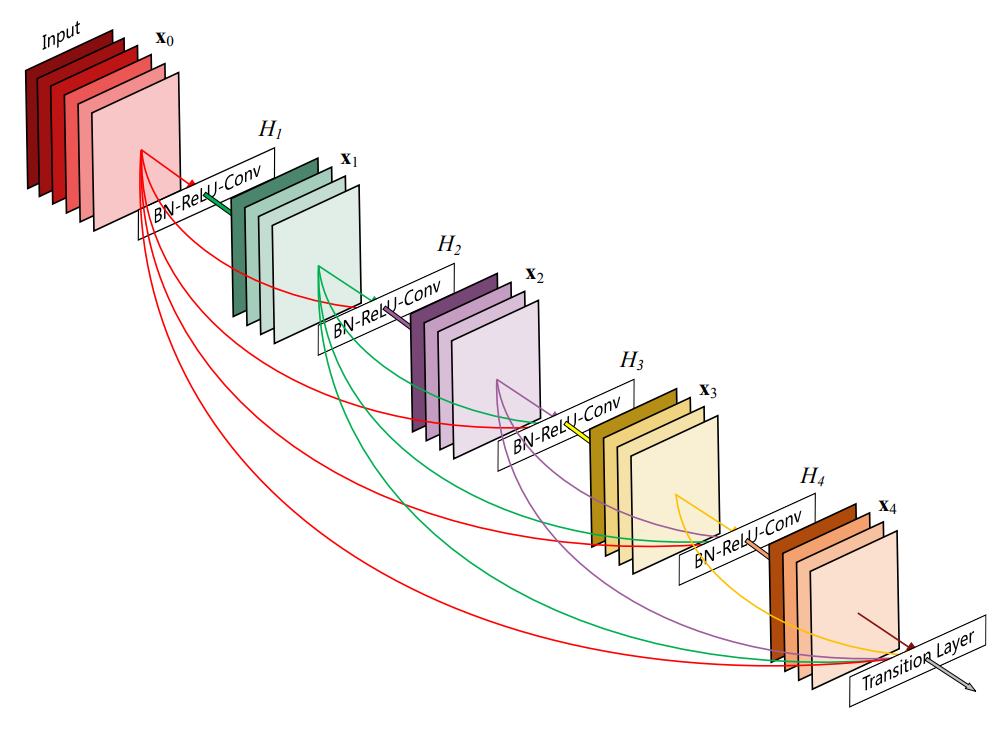
\includegraphics[width=0.70\textwidth]{2/figures/densenet_5lay.png}
		\caption[DenseNet con 5 capas]{DenseNet con 5 capas. \\
		Fuente: \cite{pr_huang2016densconn}. \textit{Densely Connected Convolutional Networks}.}
		\label{2:fig205}
	\end{center}
\end{figure}

% Las tareas relacionadas al procesamiento de imágenes como la segmentación, detección de objetos y clasificación es actualmente dominada por las redes neuronales convolucionales explicadas anteriormente; sin embargo, gracias al gran avance y divulgación de los modelos basados en Transformers, se ha visto el surgimiento de un nueva clase de arquitecturas que prometen mejorar el desempeño de los actuales modelos dominantes: los Vision Transformer (ViT).

A pesar del gran desempeño del los modelos de basados den CNN, los últimos años han aparecido nuevas y prometedoras arquitecturas capaces de superarlos.

Según la investigación original presentada por \cite{pr_dosovitskiy2021animageisworth}, los modelos Transformer, dominantes actuales en tareas de procesamiento de lenguaje natural (NLP), se han convertido en el modelo predilecto cuando se trata de manejo de texto, esto debido a su capacidad de utilizar los recursos computacionales de forma eficiente y su escalabilidad, permitiendo así obtener modelos de; por ejemplo, 100 mil millones de parámetros.

% A diferencia de las tareas de NLP, la visión por computadora tuvo mayores problemas para adaptar este nuevo tipo de arquitecturas a sus tareas específicas.

Los primeros intentos de ingreso de esta arquitectura en la visión por computadora se basaban en usar la capacidad de self-attention de los Transformer y combinarlo con los dominantes modelos CNN. Estos intentos de obtener los excelentes resultados de los Transformer en las tareas de visión por computadora no obtenían los resultados de los modelos de mayor desempeño como son los basados en la arquitectura de ResNet.

Debido a esto y al gran potencial que tenían las arquitecturas basadas en Transformers, propusieron el uso de estas arquitecturas aplicadas de forma directa a imágenes; es decir, aplicando la menor cantidad de cambios antes de ingresar al mismo Transformer. El proceso exacto de cómo funciona su arquitectura se explicará más adelante.

La gran ventaja de este nuevo tipo de modelos se basa en la cantidad de datos con la que es entrenado. 

En el caso de usar una pequeña cantidad de imágenes para el entrenamiento se obtienen resultados no favorables, llegando a tener un bajo rendimiento comparado a los modelos basados en CNN. Sin embargo, al realizar su entrenamiento con una mayor cantidad de datos, los Vision Transformer (como se le nombró a este nuevo tipo de arquitectura) obtuvieron mejores resultados que los modelos dominantes en las mismas tareas de visión por computadora.

A diferencia de los Transformer dedica a las tareas de NLP que reciben como entrada token embeddings de una sola dimensión, las imágenes son de dos dimensiones (H, W) y una cantidad de canales (C), lo que dificulta su ingreso directo a este tipo de arquitecturas. Es por esto que es necesario aplicar una división de las imágenes en patches 2D que posteriormente serán aplanados e ingresados al Transformer como haría normalmente los token embeddings.

Estos patches deben tener un tamaño constante P, es decir que se deben obtener divisiones de las imágenes de tamaño P x P. Esto conlleva a que el número de patches final sea igual a $N = HW / P^2$.

Una vez se tienen los N patches, se realiza su aplanamiento y, posteriormente, se mapean en D dimensiones (tamaño del vector latente usado en el Transformer) a través de una proyección lineal capaz de ser entrenada.

Ya obtenidos estos patch embedding, se añade uno nuevo pero con la capacidad de ser aprendible. Estos se agrupan en una secuencia que ingresarán posteriormente al Transforme encoder. Cabe resaltar que, luego de pasar por el encoder, este último embedding añadido representará a la imagen.

A los ya mencionados patch embedding también se le agrega otro tipo de embedding capaz de mantener información relacionada a la posición de cada patch. Estos embedding son 1D y aprendibles. Finalmente, estos serán ingresados juntos con los originales embeddings a Transformer encoder.

En la parte final de la arquitectura se tiene un MLP con la principal tarea de realizar la clasificación de las imágenes. Este MLP consta de una sola capa oculta en la etapa de entrenamiento inicial del modelo, y con una sola capa lineal en la etapa de fine-tuning.

El bloque de Transformer encoder está compuesto por distintos bloques como los multi headed self attention (MSA), MLP y los Layernorm (LN). Estos distintos bloques se van alternando de forma específica, introduciendo además conexiones residuales luego del MSA y MLP.

Toda la arquitectura de los ViT se puede resumir con la siguiente imagen.

\begin{figure}[H]
	\begin{center}
		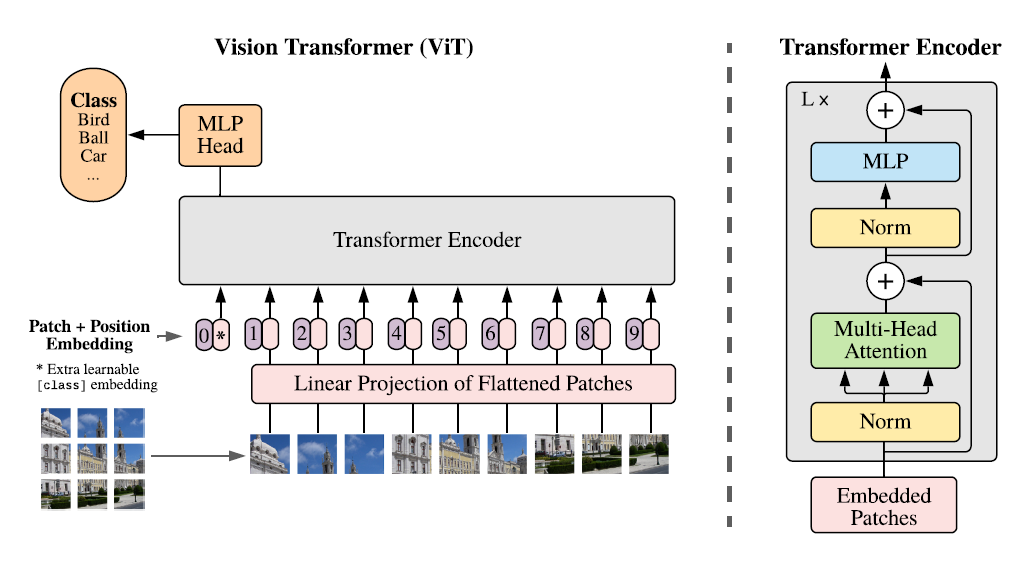
\includegraphics[width=1.00\textwidth]{2/figures/vit_arquitecture.png}
		\caption[Arquitectura del modelo ViT]{Arquitectura del modelo ViT. \\
		Fuente: \cite{pr_dosovitskiy2021animageisworth}. \textit{AN IMAGE IS WORTH 16X16 WORDS: TRANSFORMERS FOR IMAGE RECOGNITION AT SCALE}.}
		\label{2:fig206}
	\end{center}
\end{figure}


\subsection{Nódulos Tiroideos}
Para entender qué es un nódulo tiroideo, primero se debe sabes qué es la tiroides. Este es una glándula localizada en el cuello del cuerpo humano que se encarga de producir hormonas que regulan el metabolismo. Los nódulos que aparecen en esta glándula son los más comunes, y se generan debido a un excesivo crecimiento de las células en esa área, estos pueden ser de textura dura o quísticas. \parencite{pr_deng2022autclass}

La siguiente figura muestra a la glándula en una imagen tomográfica.

\begin{figure}[H]
	\begin{center}
		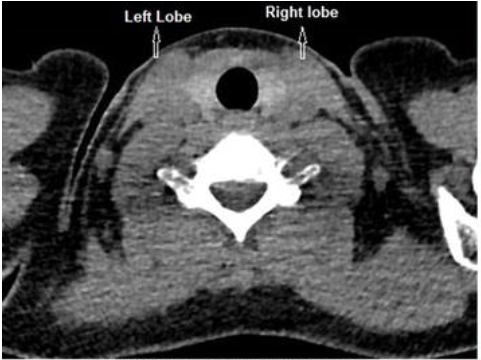
\includegraphics[width=0.55\textwidth]{2/figures/gland_thyroid.png}
		\caption[Imagen tomográfica de glándula de tiroides]{Imagen tomográfica de glándula de tiroides. \\
		Fuente: \cite{pr_binboga2019thyroid}. \textit{Thyroid Anatomy}.}
		\label{2:fig207}
	\end{center}
\end{figure}

\cite{pr_shin2016ultradiag} mencionan que existen algunas características de los nódulos en la tiroides que pueden ser analizados para realizar una clasificación si es de carácter benigno o maligno. A continuación, se presentan aquellos más resaltantes.

El tamaño de nódulos en ciertos casos puede determinar el tipo con el que se está tratando; sin embargo, esto no está debidamente comprobado, a pesar de que normalmente el riesgo de ser maligno de un nódulo es más alto en aquellos de mayor tamaño. Esto principalmente se debe a que los nódulos benignos también pueden llegar a un tamaño considerable, pero con una mayor cantidad de tiempo. Lo que sí puede significar un probable nódulo maligno es un rápido crecimiento de un nódulo sólido.

El contenido interno de un nódulo está determinado por el ratio entre su parte quística y su parte sólida. Los nódulos malignos con contenido sólido poseen mayor riesgo de ser malignos que aquellos con contenido parcialmente quístico.

La ecogenicidad de los nódulos se mide de acuerdo al nivel de brillo en las imágenes de ultrasonido con respecto a otras partes de la imagen. Esto quiere decir que un nódulo es hipoecoico si su nivel de brillo en la imagen es menor con respecto a otra parte de la imagen, específicamente se compara con el músculo anterior del cuello o el parénquima tiroideo. La mayoría de los tumores tiroideos son hipoecoicos, y existe mayor riesgo de que los nódulos con la misma característica sean malignos.

La forma y orientación de los nódulos también pueden determinar si son o no malignos. La manera en que los nódulos malignos crecen es de manera centrífuga y a través del plano del tejido, al igual que los benignos; sin embargo, estos crecen de manera paralela. La forma redonda u ovoide de los nódulos se encuentra en aquellos de carácter benigno; sin embargo, no son propias de este. Una característica mucho más específica de los nódulos de carácter malignos es su orientación no paralela, es decir, son más altos que anchos.

Finalmente, el margen de los nódulos también puede dar información del tipo con el que se trata. Una característica que sugiere que un nódulo es maligno es un margen espiculado o micro tubulado.

